\chapter{User sessions}
\section{Prototypes - Theis}
In order to get information from the users about how the user interface should be like six sessions were made with different purpose and users. For the user sessions four prototypes were made, the prototypes is as follows.

\subsection{Hub low fidelity}
The low fidelity hub prototype is used in the participatory design session. The prototype is a box with an aluminium sheet as front, this should act like the hub, then pictures of different types of components were printed out, such as bottoms, LEDs and screens. This makes it easy to rearrange the design, just by moving the pictures around the front sheet. This is a low fidelity prototype, because it do not do anything functional, it is to show how the design could turn out.
\begin{figure}[H]
	\center
		\setlength\fboxsep{0pt}
		\setlength\fboxrule{1pt}
		\fbox{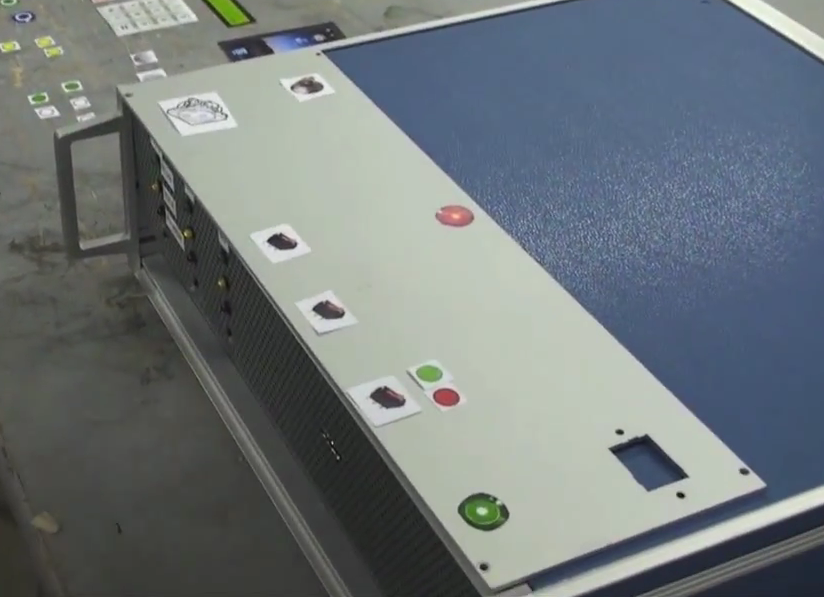
\includegraphics[width=0.7\textwidth]{images/LF_hub.png}}
   	\caption{Picture of the hub LF after session}
   	\label{fig:LF hub after session}
\end{figure}

\subsection{Hub high fidelity}
The high fidelity hub prototype was made before the participatory design session, and this was how his needs was defined. The prototype is also used in the participatory design. It were made with the same box as the low fidelity hub prototype, an mbed were used to control the LEDs and bottoms in the front sheet. This is a high fidelity prototype, because it can show how the hub will react on different actions, it gives the user the same experience as a fully operational hub would with this user interface.
\begin{figure}[H]
	\center
		\setlength\fboxsep{0pt}
		\setlength\fboxrule{1pt}
		\fbox{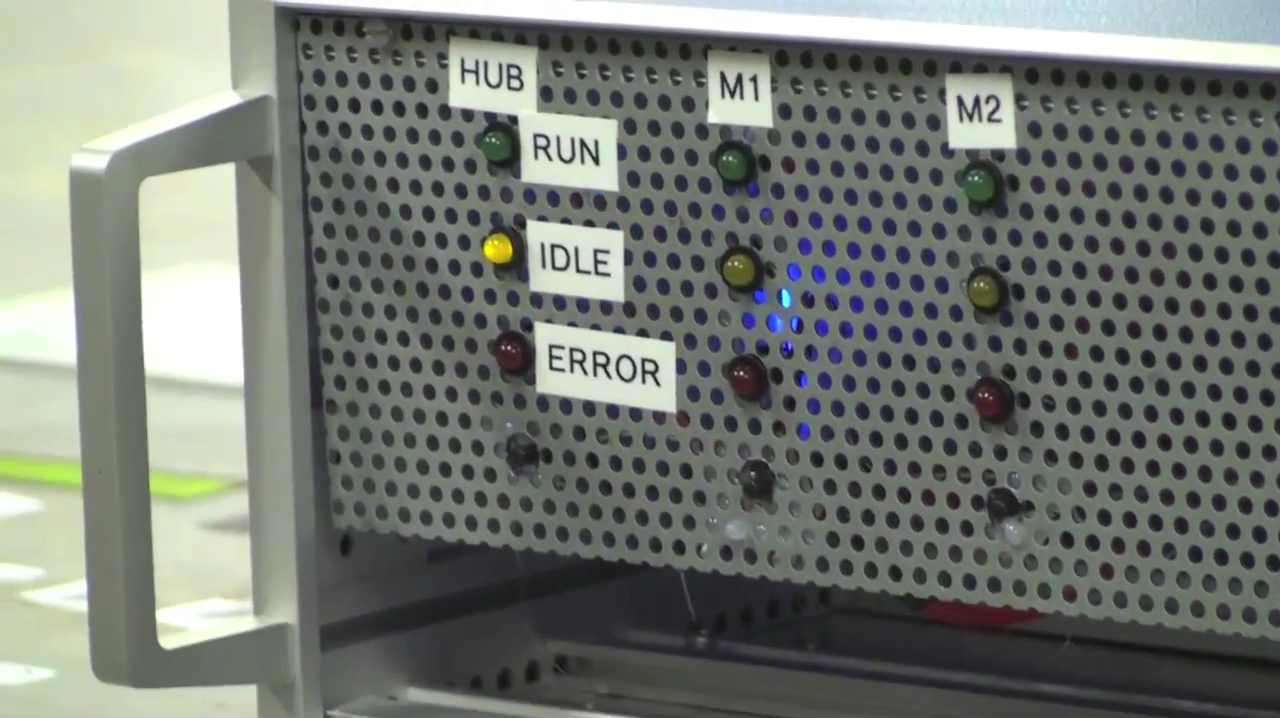
\includegraphics[width=0.6\textwidth]{images/HF_hub.png}}
   	\caption{Picture of the hub HF}
   	\label{fig:High fidelity hub}
\end{figure}

\subsection{Power point mid fidelity}
The power point prototype is used in the first usability test. It is an interactive power point with slides to show the different web pages, it is said that this is a mid fidelity prototype, it gives the user a good experience as the final page would do, but it dose not have any dynamic data, it is all static so that it is just to see how the interaction with the page works.
\begin{figure}[H]
	\center
		\setlength\fboxsep{0pt}
		\setlength\fboxrule{1pt}
		\fbox{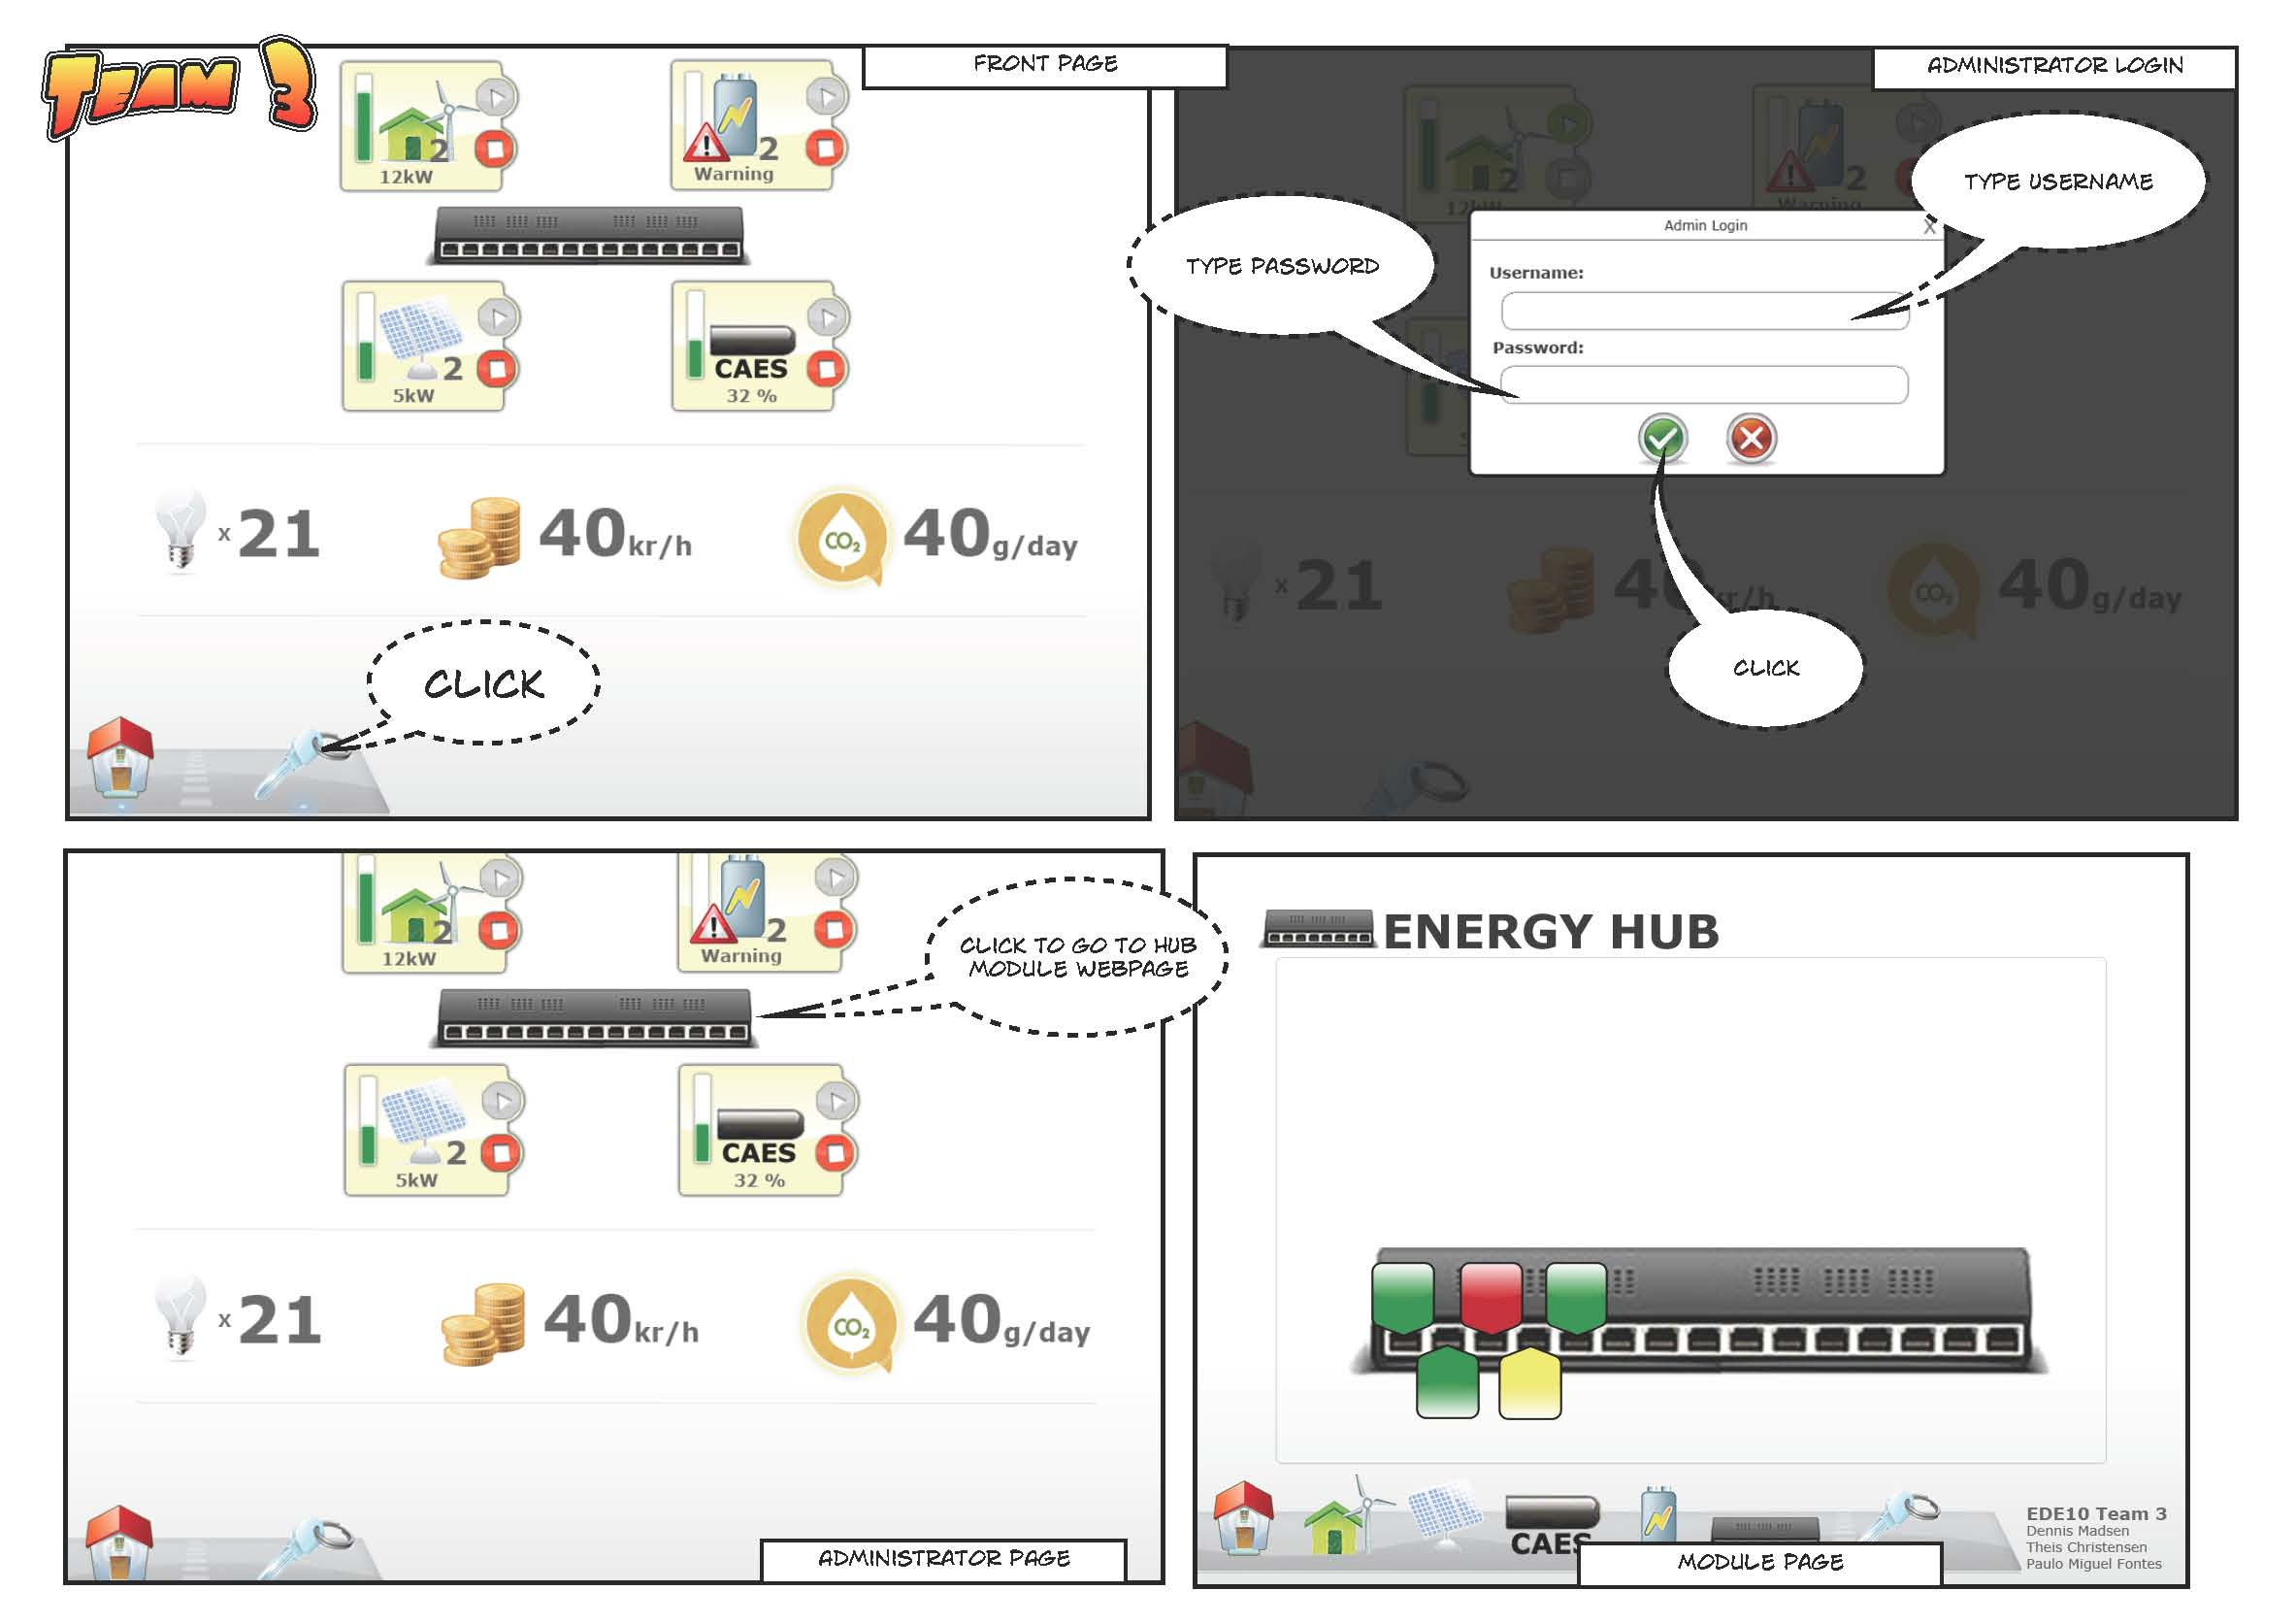
\includegraphics[width=0.6\textwidth]{images/web_interface1.jpg}}
   	\caption{Picture of the power point slides}
   	\label{fig:web_interface1}
\end{figure}

\subsection{HTML web page mid fidelity}
The HTML page prototype is used in the second usability test. It is the web page developed in EWEB1 course, the purpose of the site is to give at picture of how the final web page would look like and work but without any data reading and logging, it is a static web page. It is said this to be mid fidelity as the power point because it perform the same purpose and have the same functionality.
\begin{figure}[H]
	\center
		\setlength\fboxsep{0pt}
		\setlength\fboxrule{1pt}
		\fbox{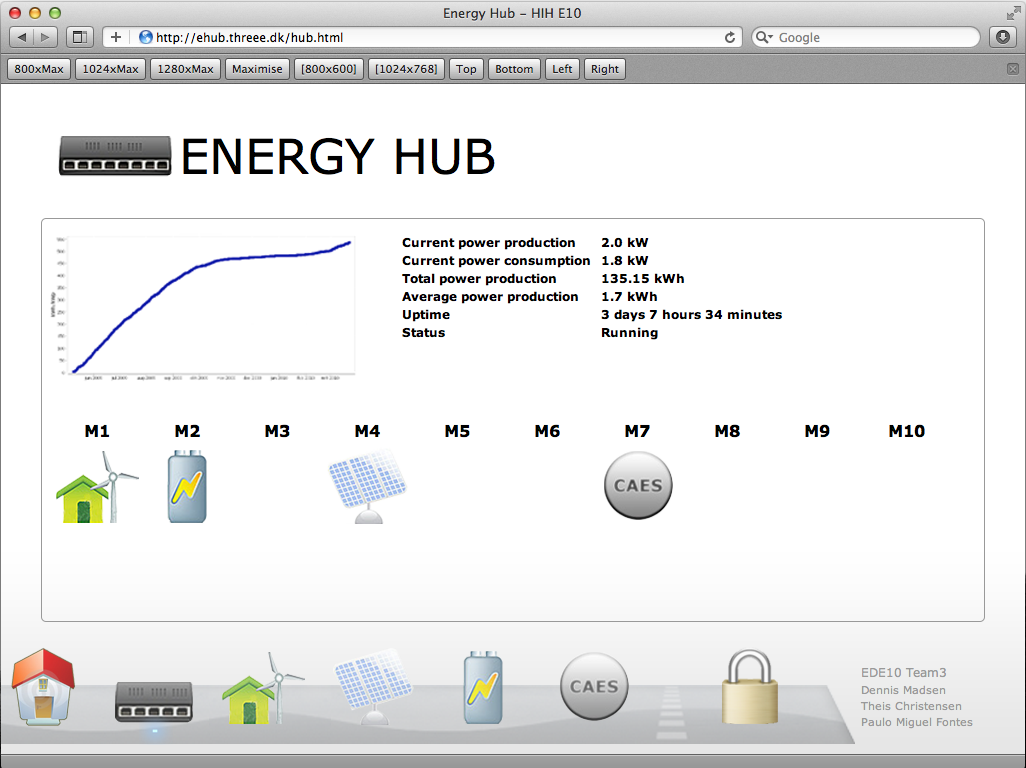
\includegraphics[width=0.6\textwidth]{images/screen_hub_page.png}}
   	\caption{Picture of the hub web page}
   	\label{fig:web_hub_interface}
\end{figure}
\begin{figure}[H]
	\center
		\setlength\fboxsep{0pt}
		\setlength\fboxrule{1pt}
		\fbox{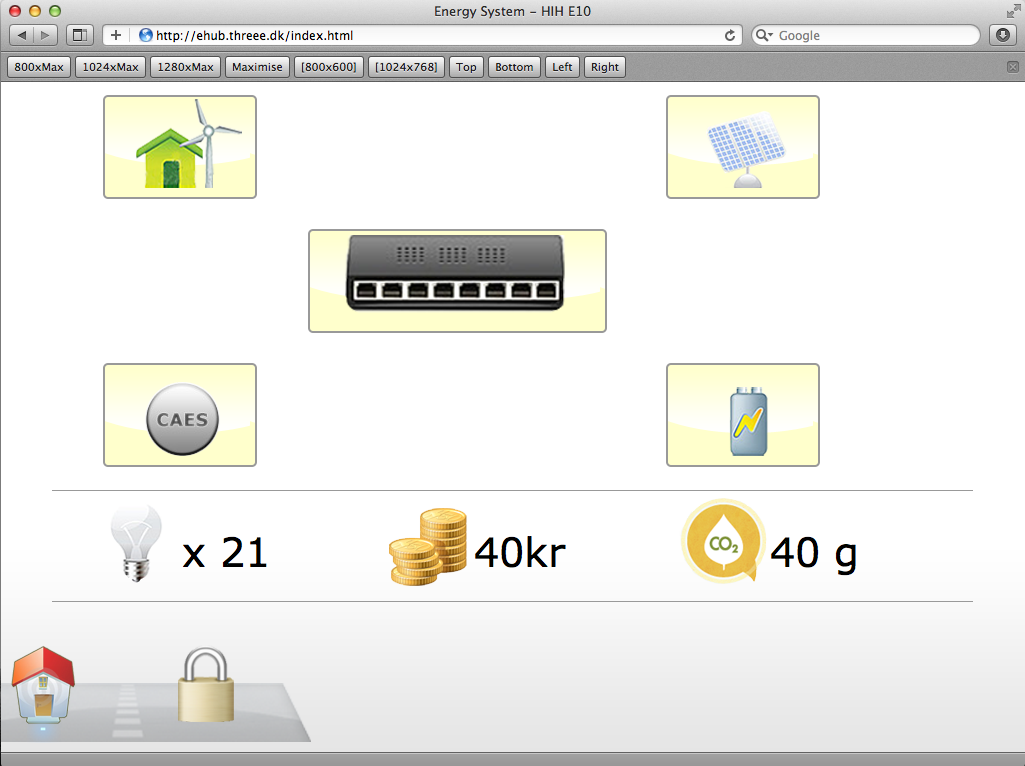
\includegraphics[width=0.6\textwidth]{images/screen_index_page.png}}
   	\caption{Picture of the index web page}
   	\label{fig:web_index_interface}
\end{figure}
%%%%%%%%%%%%%%%%%%%%%%%%%%%%%%%%%%%%%%%%%
\section{Participatory Design - Dennis}
As explained earlier, the hub module is divided into two sections, the web interface and the physical interface on the hub. 
The goal of the participatory design session with the customer Jan was to clarify the level of interaction he wants on the hub module, but also where he wants the different things to be placed. A video of the session can be found on the wiki page (find link in the introduction section). Before the session, pictures of small buttons, LED's, screens, connecters etc. were printed out to easy to process of placing components on the front panel. Jans job was now, with some guidance instructions, to place the components he wanted on the hub and where he wanted them. The design ended up with a clean design containing: 
\begin{itemize}
	\item 1 Power button, to turn on the hub. The button should have built in LED.
	\item 1 emergency button (powers off everything).
	\item 1 on/off switch for each module (position switch).
	\item 2 indication LED for each module (green on = module is powered on. Red on = module is powered off).
	\item A 230VAC plug is placed on the front to connect: light, phone-chargers or similar. 
\end{itemize}
To get access to the front panel of the hub, a locker have to be opened with a key, to protect agains fiddle-fingers. The emergency button is of cause operational all the time and no locker needs to be opened to use it.
\\When finishing his idea about the front panel of the hub, Jan was introduced to another solution, which worked as a prototype of the finish product. Jan was asked to go through some tasks:
\begin{itemize}
	\item Turn on the hub.
	\item Connect a module.
	\item Turn on the connected module.
	\item Identify an error on a module.
	\item Repair the module.
	\item Shut down the system.
\end{itemize}
The general impression from Jan was positive, but some of the functions found on the interface was unnecessary as he will primarily use a PC to check the status of the different devices (on the web interface). The placement and method of connecting new devices was fine and the same with turning on and off the hub. Instead of the pushbuttons found on the prototype, as mentioned, he wanted position switches. The indication of every module was fine, but unnecessary indicators should be removed. 
%%%%%%%%%%%%%%%%%%%%%%%%%%%%%%%%%%%%%%%%%
\section{First usability tests - Theis}
In the first usability test, the power point were used as a demonstration prototype of the web page. There were made two sessions, one with Rene and one with Jan as the web customer and the full system customer. A camera were used to record the actions on the screen, and another to record the face expressions. In the sessions Rene and Jan had free hands to play around with the power point. The goal of this test was most of all to show the design, and then get some reactions and comment on what was good and what was bad. There was no specific tasks that the users should do, so this was not completely a usability test. Both Rene and Jan was positive surprised, but they had also a lots of things that they would have on the final page.\\\\
\textbf{Rene would like:}
\begin{itemize}
	\item Identify modules - Give an ID for each modules so they can be identified easily
	\item Warnings - Optimise warning status for a more intuitive experience (maybe change background of the icon)
	\item Graphs - Make the graphs full screen when click on
	\item Permissions - User without log in should be allow to see everything but not change it
	\item Status - Make vertical bar more intuitive, add colour scheme to it (red, yellow, green)
	\item Update - The data should update every 5 to 10 seconds
\end{itemize}
\textbf{Jan would like:}
\begin{itemize}
	\item Small data font - Make bigger data text
	\item Explanation for graphs - Make a small explanation for what the graphs shows
	\item Graphs - Make the graphs full screen when click on
	\item Energy for storage device - Show the energy for storage modules for comparing with other modules
	\item Start/Stop - The start and stop function for the modules did not work intuitive for him
	\item Not exciting - The page was a bit boring
\end{itemize}
In the development of the final web page, with all the PHP and dynamic integration, every suggestion from the two sessions will be considered. Identifying the modules will be taken care of with the PHP, so when you click the wind turbine and there is more than one of them, every module will be shown with there ID so the user easily can figure out what module he wants to look at.\\
The warnings should be more visible, Rene suggested to maybe change the background color of the module when there is an error. This observation got supported very well in the session with Jan, he did not notice that there was an error on one of the batteries, warnings will be made more visible on the final page, and maybe use the suggestion from Rene with the background color.\\
Both Jan and Rene wanted to make the graphs full screen when they click on them, this will also be implemented in the final page, maybe with a page where the user can change settings for the graphs and see explanation for what the graph shows.\\
The permissions for users without log in, is already implemented in the HTML page, so it is possible to see everything on the page without having to log in, but for the possibility to change things you have to log in, this will be made on the final page.\\
They both wanted more data on the modules, and comparison options between the modules, and the specification of the modules, this will be implemented on the final page, when it is possible to get all data through PHP implementation.\\
Rene wanted the data to update every 5 to 10 seconds, this would be waste of resources if no one is looking at the web interface, to optimize this, the web interface would check if anyone is using the page, if someone is using it the data will be updated from the log every 5 - 10 seconds.\\
Jan said that the font was a bit small, this will be helped so it is easy to change the text size on the page.\\
Jan also said that the page was not exciting, and suggested to use more color, It is because of the page is static, in the final page there will be used java scripting to make effect and animation on the page, this will help on the excitement for the web page.\\
Jan did not think our start and stop bottoms was intuitive, because of the colors and there was no clearly status indication of the single module, this will be made with a status box for each module clearly showing the status of the module.\\
Lots of feedback were given on the design from the two sessions, and the plan is to implement all of them in a way so it will fulfil the feedback from Rene and Jan. There was no very big things they wanted, so it is all small things that they think would help on the user experience. This is why it is a good idea with user sessions, a better understanding of the user needs and concrete suggestion to changes that would make the interface better, this makes it easy to implement because the exact needs is know.


%%%%%%%%%%%%%%%%%%%%%%%%%%%%%%%%%%%%%%%%%
\section{Second usability tests - Paulo}

In this usability test, persons with different interests and knowledges were selected, a wide different feedback can be acquired, such as: user experience and how persons with different backgrounds interact with the interface.
\\
\\Two different categories where selected to this usability test:\\
- 1 Person directly involved on the project.\\
- 4 Persons with no involvement, or overview over the project.\\
\\

The evaluation will be made on the performance, accuracy and emotional response while the user is interacting with the system, the sessions were recorded for later analysis.

In the performance, the system will be evaluated in how much time and how many steps until the user finish simple tasks. Accuracy is determine by the number of mistakes the user have until finish the task, in emotional response the users actions, thoughts about the system and what feelings they got when fulfilling all tasks will be considered.
\\
5 simple tasks were asked from the users:\\
- Unlock the system.\\
- View photovoltaic average power production .\\
- See the current power production on the energy hub.\\
- Find the current status on the battery module.\\
- Lock the system.\\

\subsection{Setting the Scene - Paulo}
Setting up a usability test requires the creation of a real scenario (hi-fidelity prototype), in this case a real webpage. User could navigate in the system and since everything was recorded, data can be extracted later on, without compromising any of the user thoughts when interacting with the web interface.

The aim of this usability test is to observe how users interact with the navigation in a realistic way, so developers can understand problematic areas in the design and be able to improve the interface.

This usability test was performed with students from AU-Herning, with and without any knowledge for the system. The use of a laptop with the web interface running on a web browser and the use of a mouse or trackpad. The session was recorded, with authorisation from the user, this was performed by the front camera and screen capture, in this manner the reactions from the users could be recorded while interacting with the system.

\subsection{Testing and results - Paulo}

The results of the usability tests are describe below:

\begin{table}[H]
	\begin{tabular}{ | l | l | l | l |}
		\hline
		Task 				 	     & 		Time 	& 	Steps 	& 	Mistakes 		\\ \hline
		Unlock the system    			     & 		20s  		& 	 5 		& 	1 			\\ \hline
		Photovoltaic avr. pwr. production  & 		10s 		& 	 1 		& 	0 			\\ \hline
		Energy hub current production 	     & 		7s 		& 	 1 		& 	0			 \\ \hline
		Current status battery module 	     & 		6s 		& 	 1 		& 	0 			 \\ \hline
		Lock the system 			     & 		2s 		& 	 1 		& 	0 			 \\ \hline
	\end{tabular}
    \caption{Person directly involved on the project. Usability Test \#1}
\end{table}

The first user, was a person directly involved on the green energy system. The system worked as expected for the user, he was able to complete the task easily and without any troubles, some functionalities should be improved/implemented:\\
- Unlocking the system, it requires a click on the 'OK' button to submit the credentials. May be useful to implement a key press 'enter' to submit the user and password, since this is how most users are used to work on the internet and different OS's.\\
- A small explanation of "Savings" icons on the front will be implemented, the user tries to click on them to get more information, without any success.\\

\begin{table}[H]
	\begin{tabular}{ | l | l | l | l |}
		\hline
		Task 					     & 		Time 	& 	Steps 	&	 Mistakes \\ \hline
		Unlock the system 			     & 		20s 		&	 5 		& 		0 	\\ \hline
		Photovoltaic avr. pwr. production  & 		22s 		& 	 1 		& 		1 	\\ \hline
		Energy hub current production 	     & 		16s 		& 	 3 		& 		2 	\\ \hline
		Current status battery module 	     & 		7s 		& 	 1 		& 		0 	\\ \hline
		Lock the system 			     & 		4s 		& 	 1 		& 		0 	\\ \hline
	\end{tabular}
     \caption{Persons with no involvement, or overview over the project. Usability Test \#2}
\end{table}

In this usability test, a person with no knowledge about energy or any overview of the project, was selected. This can be compared to the High School students that will see the system for the first time.\\
Some improvements taken from this test is:\\
- When the user was asked to see the solar panel (photovoltaic) average production, there were difficulties to associate the icon to the name of it.\\
- The user have many troubles to identify the energy hub icon in the bottom menu, this will be improved so the navigation in the system would be easier.\\

\begin{table}[H]
	\begin{tabular}{ | l | l | l | l |}
		\hline
		Task 					      & 	Time 	& 	Steps 	& 	Mistakes  \\ \hline
		Unlock the system 			      & 	22s 		& 	1 		& 	0 		\\ \hline
		Photovoltaic avr. pwr. production   & 	9s 		& 	1 		& 	0 		\\ \hline
		Energy hub current production 	      & 	16s 		& 	1 		& 	0 		\\ \hline
		Current status battery module 	      & 	5s 		& 	1 		& 	0 		\\ \hline
		Lock the system 			      & 	6s 		& 	1 		& 	0		\\ \hline
	\end{tabular}
    \caption{Persons with no involvement, or overview over the project. Usability Test \#3}
\end{table}

A person with no knowledge about energy or any overview over the project was selected. From this usability, the user have difficulty on finding the energy hub on the bottom menu, this can be a big issue in the navigation of the system. 

\begin{table}[H]
\begin{tabular}{ | l | l | l | l |}
	\hline
	Task 					     &		Time 	& 	Steps 	& 	Mistakes 		\\ \hline
	Unlock the system 			     & 		21s		& 	1		& 	0			\\ \hline
	Photovoltaic avr. pwr. production  & 		11s		&	1		& 	0			\\ \hline
	Energy hub current production      & 		13s		& 	1		& 	0			\\ \hline
	Current status battery module 	     & 		5s		& 	1		& 	0			\\ \hline
	Lock the system 			     & 		4s		& 	1		& 	0			\\ \hline
\end{tabular}
\caption{Persons with no involvement, or overview over the project.  Usability Test \#4}
\end{table}

In this usability test the association between the names and the icons is hard to understand for the user. This will be improved, since the user experience and navigation are being affected.\\

\begin{table}[H]
\begin{tabular}{ | l | l | l | l |}
	\hline
	Task 					      & 	Time 	& 	Steps 	& 	Mistakes 		\\ \hline
	Unlock the system 			      & 	38s		& 	1		& 	0			\\ \hline
	Photovoltaic avr. pwr. production   &		4s	    	& 	1		& 	0			\\ \hline
	Energy hub current production 	      & 	41s		& 	5 		& 	4 			\\ \hline
	Current status battery module 	      & 	4s		& 	1		& 	0			\\ \hline
	Lock the system 			      & 	3s		& 	1		& 	0			\\ \hline
\end{tabular}
\caption{Persons with no involvement, or overview over the project. Usability Test \#5}
\end{table}

The user feels confused when asked to perform the first task, the amount of icons in the front screen makes it confusing since the user doesn't now which ones are selectable. The energy hub icon is not associated with its name, making the user getting lost in the navigation, this could be avoid having a short name of the module on mouse over.

\begin{figure}[H]
	\center
		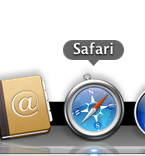
\includegraphics[width=0.2\textwidth]{images/legend.png}
   	\caption{Apple solution}
\end{figure}

\subsection{Usability Tests Analysis - Paulo}

The performance and accuracy retrieved by the usability tests are showed below:\\
	
\begin{table}[H]
\begin{tabular}{ | l | l | l |}
	\hline
	Task 					      & 	Performance 	& 	Accuracy 		\\ \hline
	Unlock the system 			      & 	24.2s		& 	9			\\ \hline
	Photovoltaic avr. pwr. production   &		11.2s	    	& 	9			\\ \hline
	Energy hub current production 	      & 	18.6s		&	6 			\\ \hline
	Current status battery module 	      & 	5.4s			& 	10			\\ \hline
	Lock the system 			      & 	3.8s			& 	10			\\ \hline
\end{tabular}
\caption{Accuracy ( 10 - Higher accuracy, 0- Lower accuracy ) and Performance (time average in seconds per task), data retrieved by the usability tests.}
\end{table}

Task \#1: to unlock the system the user have to type the user name and password on two text fields, this was performed without any difficulty and the time was similar in the first 4 tests, just one user had more difficulties to find  the unlock icon, since it was confusing all the icons on the front page. The key 'enter', would be a good implementation since it is used by many users in the tests.\\
\\
Task \#2: when users were asked to see the solar panel (photovoltaic) average production, there were difficulties to associate the icon to the module name. A label with the name of the module will be useful to guide to the right module.\\
\\
Task \#3: this task was the most problematic for all the users without any knowledge about the energy system. In this task the accuracy drops o 6, this reflects the higher difficulty in this task for most of the users. This can be improved by writing labels with the name next to the icon of the module.\\
\\
Task \#4: there were no difficulties with this task, all users could easily associate the battery icon with his name. This was perfumed with 10 of accuracy.\\
\\
Task \#5: there were no difficulties with this task, it was performed by all users with success.\\
\\
Usability tests at this initial phase of the project were the most useful feedback, since a navigation, as developers were easy to understand and follow, for users was confusing and sometimes even problematic.

Further improvements are going to be implemented to the web interface, so the users would be able to interact with the system easily and without any problems. \\
\begin{itemize}
	\item Further implementation on navigation system:
		\begin{enumerate}
			\item Implement a key press 'enter' to submit the credentials.
			\item A small explanation of "Savings" on front page will help the user experience.
			\item The amount of icons in the front screen makes it confusing since the user doesn't now which ones are selectable.
			\item  A label with the name of the module will be implemented to guide the user.
		\end{enumerate}
\end{itemize}

Usability tests are going to be performed in next phases of the project, since the goal of the web interface is the user and the interaction with the system. In further usability tests, high school student may be invited, since they are focus group of users that will use the web interface.

%%%%%%%%%%%%%%%%%%%%%%%%%%%%%%%%%%%%%%%%%%%%%%%%%%%%%%%%%%

\section{Drama - Theis}
A drama play is a good tool for engaging a user as co designer in a project. It is always a good idea to involve the user in development of the product, because they will be using the final product and can easily help with designing the product. This can be accomplished with a drama play, a good thing about the drama play, is that the user is involved, it is easier for the user to understand how the technologies works, and how the product would work. It is also good for the designer because designers do not just develop a product, but also a new work station, this is why it is a good idea to involve the user. The user knows the work practices, he can imagine how he would use it, and assess changes. A drama play do not require big acting potential, it is a basic performance, to show the user how it works, and the designer how the user wants to use it. The goal of a drama session is not to entertain but to clarify how it all would be used.

\subsection{The protocol - Dennis}
All 'E-teachers' and the three web-costumers was invited to come by and witness a drama session, showing the data handling in the energy system. The session was made to clarify how the protocol in the system is going to work and find possible leaks in it. 
\begin{figure}[H]
	\center
		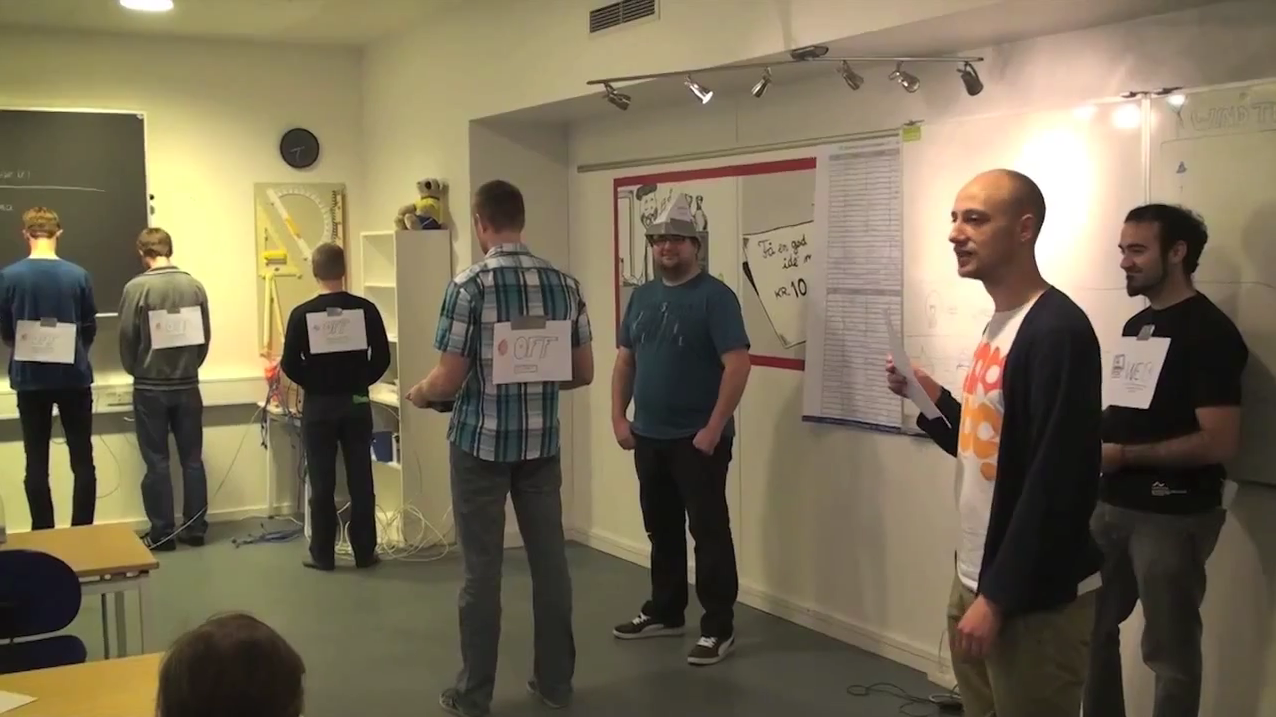
\includegraphics[width=0.7\textwidth]{images/drama_setup.png}
   	\caption{The drama session setup}
   	\label{fig:drama_session_setup}
\end{figure}

The session was divided in three scenes:
\begin{itemize}
	\item Scene 1:
		\begin{enumerate}
			\item Power on the hub.
			\item Connect two modules to the hub.
			\item Power on the modules on the hub.
			\item Start the modules on the web-interface.
		\end{enumerate}
	\item Scene 2:
		\begin{enumerate}
			\item Go to the wind-turbine page on the web-interface.
			\item Watch the graph being updated.
		\end{enumerate}
	\item Scene 3:
		\begin{enumerate}
			\item Watch what is happening if two modules sends at the same time.
		\end{enumerate}
\end{itemize}

A random person was selected from the audience (teacher Klaus Kolle) who was then supposed to go through the above mentioned steps. 

\begin{figure}[H]
  \centering
  \subfloat[Web interaction]{\label{fig:drama_web}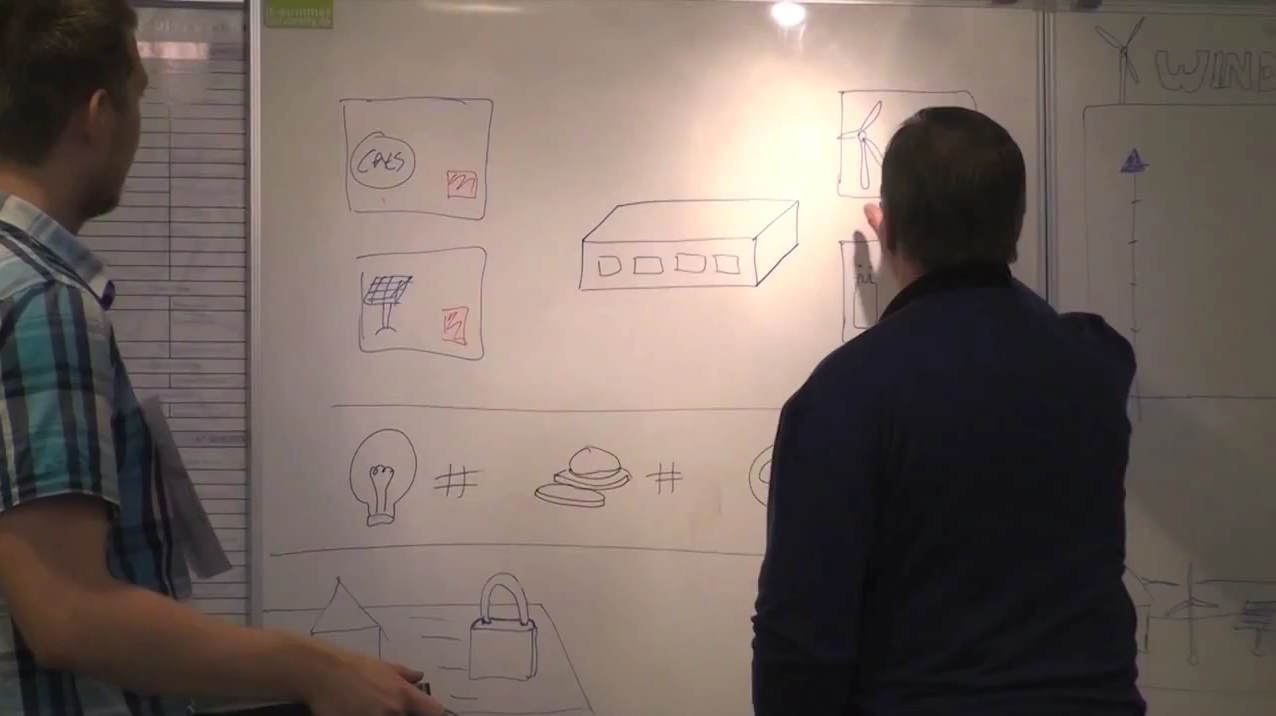
\includegraphics[width=0.45\textwidth]{images/drama_web_interaction.png}}
  \hspace{0.2cm}                
  \subfloat[Web interface]{\label{fig:drama_web}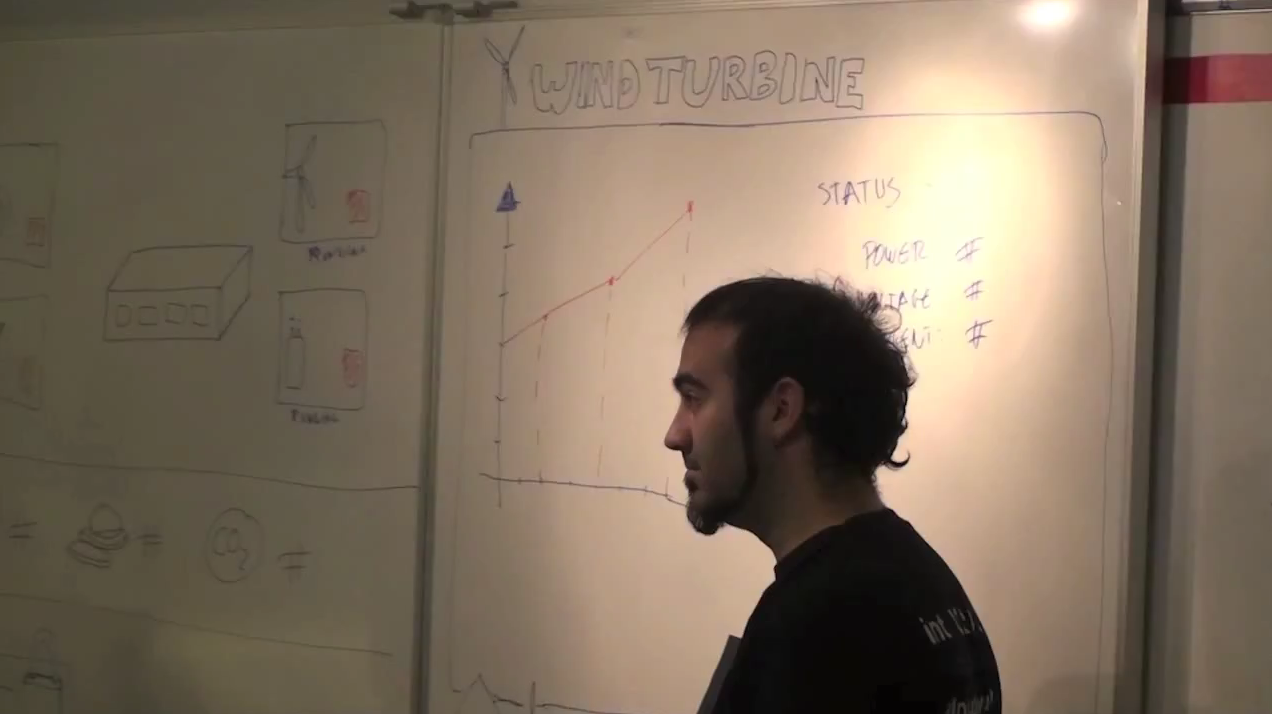
\includegraphics[width=0.45\textwidth]{images/drama_web.png}}
  \caption{Person interacting with the web interface}
  \label{fig:drama_web}
\end{figure}

A video from the drama session can be found on the wiki (find link in the introduction section).
\\[0.2cm]
After the session, the audience where asked to give some feedback. A few mistakes were found in the protocol, such as: non-defined timeout period (the amount of data delivery tries before it is seen as an error), how often data is sent, acknowledge bit check on the ethernet connection to the server and an undefined size of the data sent from the modules. 

\begin{figure}[H]
  \centering
  \subfloat[Data sent from hub to web]{\label{fig:drama_data}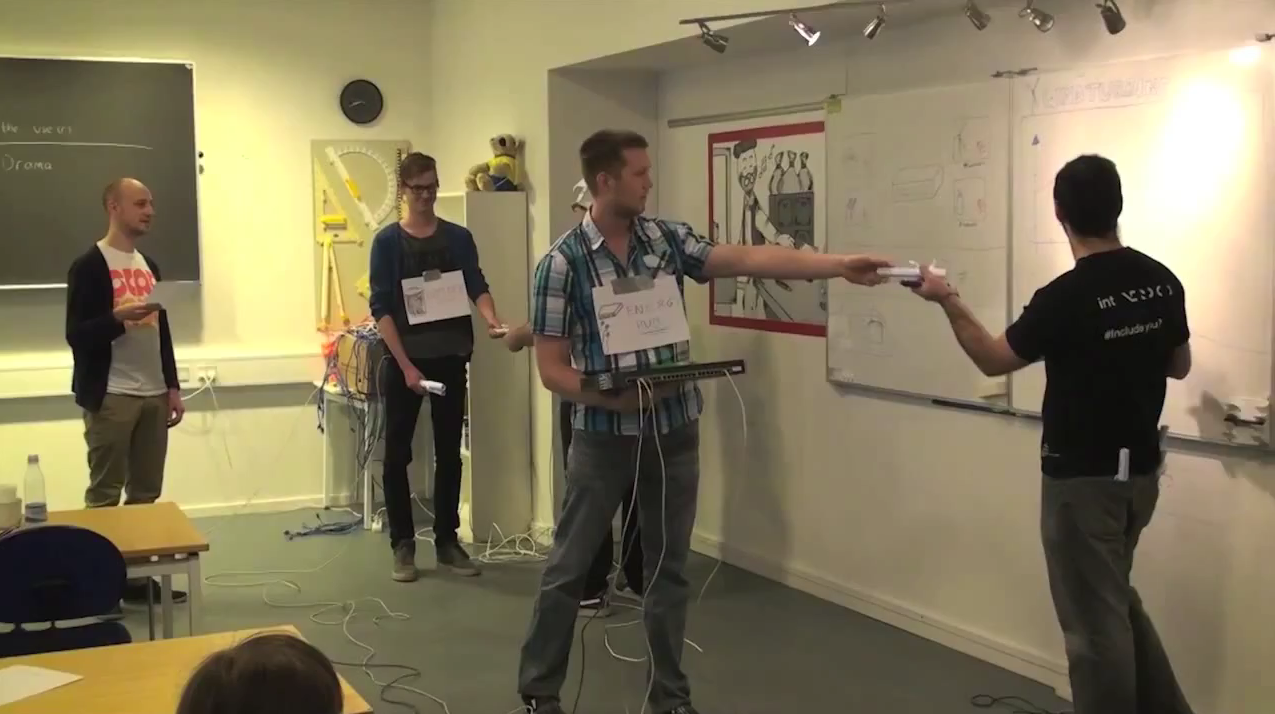
\includegraphics[width=0.45\textwidth]{images/drama_data_hub_to_web.png}}
  \hspace{0.2cm}                
  \subfloat[Web updated]{\label{fig:drama_web_update}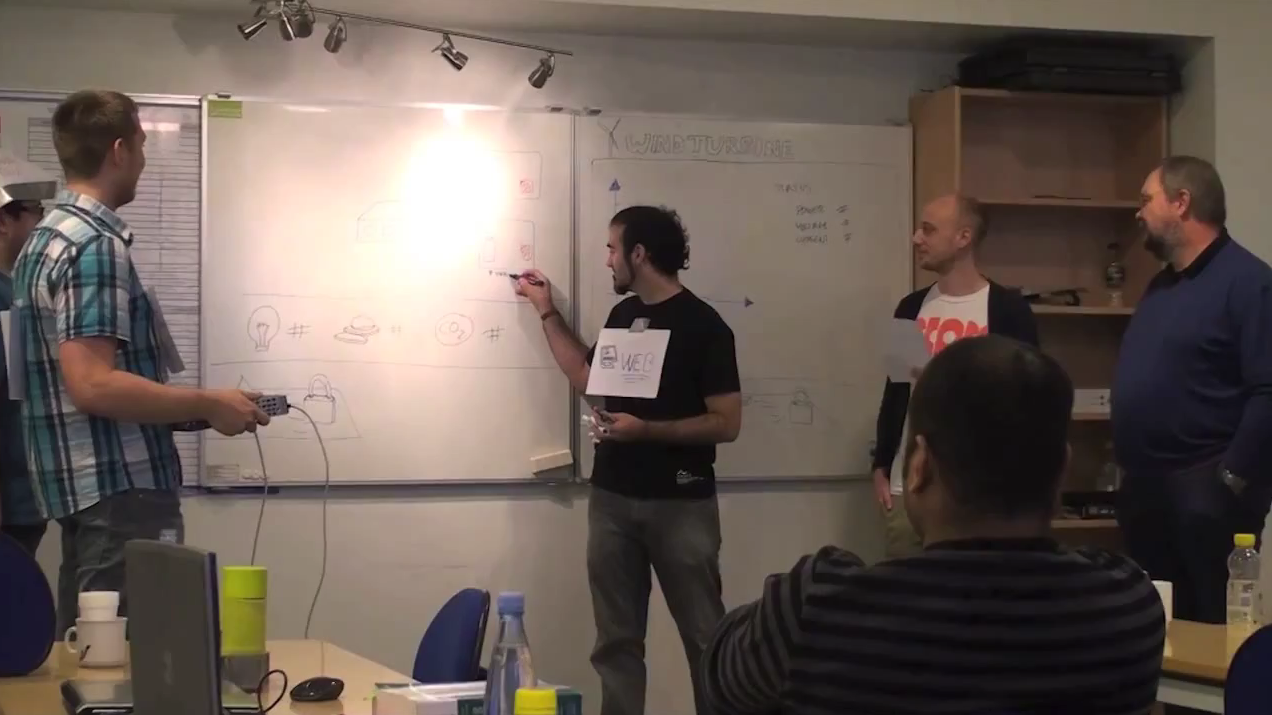
\includegraphics[width=0.45\textwidth]{images/drama_web_update.png}}
  \caption{Data sent to web interface}
  \label{fig:drama_data_to_web}
\end{figure}

As all 7 groups in the EDE10 class are part of one system, it was obvious to have one drama session with participants from all groups. The session turned out surprisingly well, especially because of the attendance from the Web-customers and the teachers who where able to see things on an early stage in the developing of the protocol that had not been thought about. These inputs will hopefully decrease the amount of protocol versions it takes to reach the final one.

